%!TEX root = main.tex
\begin{questions}

\question If after \SI{5}{\second} have passed, \SI{15}{\coulomb} has entered a terminal, determine the amount of current flowing.
\begin{solution}[\stretch{1}]
	\begin{equation*}
	\begin{split}
		I & = \frac{Q}{t}\\
		& = \frac{15}{5}\\
		& = \SI{5}{\ampere}
	\end{split}
	\end{equation*}
\end{solution}


\question Consider the time varying current leaving a terminal, modelled in Figure~\ref{fig:Q2CurrentTime}.
\ifprintanswers\else
\begin{center}
	\begin{tikzpicture}
    \begin{axis}[	xmin=0, ymin=0, xmax=5, ymax=30,
    				xlabel={Time (\si{\second})}, ylabel={Current (\si{\ampere})},
    				legend pos=north west,]
        \addplot[color=blue, domain=0:5, smooth] {3*(x-2)^2};
        \legend{$3(x-2)^2$}
    \end{axis}
	\end{tikzpicture}
	\captionof{figure}{}
	\label{fig:Q2CurrentTime}
\end{center}
\fi


\begin{parts}
	\part Determine the amount of charge transferred between $t=1$ and $t=3$ seconds.
	\begin{solution}[\stretch{1}]
		\begin{equation*}
		\begin{split}
			Q & = \int^{t_2}_{t_1}i(t)\dd{t}\\
			& = \int^3_1 3(t-2)^2\dd{t}\\
			& = 3\int^3_1 t^2-4t+4\dd{t}\\
			& = 3\left[\frac{t^3}{3}-2t^2+4t\right]^{t=3}_{t=1}\\
			& = 3\left[\left(\frac{27}{3}-2\cdot9+4\cdot3\right)-\left(\frac{1}{3}-2+4\right)\right]\\
			& = \SI{2}{\coulomb}
		\end{split}
		\end{equation*}	
	\end{solution}
	\part Determine the number of electrons that have left the terminal between $t=1$ and $t=3$ seconds.
	\begin{solution}[\stretch{1}]
		\begin{equation*}
		\begin{split}
			\text{No. of electrons} & = \frac{C}{\text{Charge of electron}}\\
			& = \frac{2}{\num{1.602e-19}}\\
			& = \SI{1.25e-19}{electrons}
		\end{split}
		\end{equation*}
	\end{solution}
\end{parts}
\newpage

\question Given Figure~\ref{fig:Q3ChargeTime}, sketch the corresponding graph for current as a function of time for the interval between $t=0$ to $t=12$ seconds.
\ifprintanswers\else
\begin{center}
	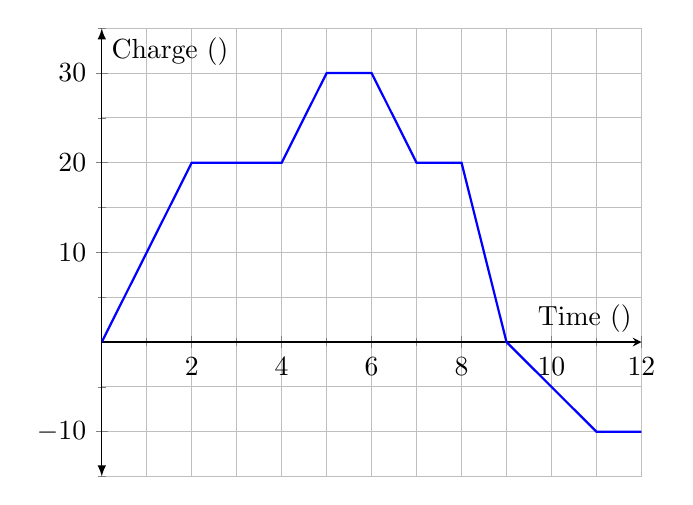
\begin{tikzpicture}[
		declare function={
			func(\x) = (\x < 2) * (10*\x)
			+ and(\x >= 2, \x < 4) * (20)
			+ and(\x >= 4, \x < 5) * (10*\x-20)
			+ and(\x >= 5, \x < 6) * (30)
			+ and(\x >= 6, \x < 7) * (-10*\x+90)
			+ and(\x >= 7, \x < 8) * (20)
			+ and(\x >= 8, \x < 9) * (-20*\x+180)
			+ and(\x >= 9, \x < 11) * (-5*\x+45)
			+ (\x >= 11) * (-10)
			;
		}
	]
    \begin{axis}[	xmin=0, ymin=-15, xmax=12, ymax=35,
    				xlabel={Time (\si{\second})}, ylabel={Charge (\si{\coulomb})},
    				legend pos=north west, 
    				domain=0:12,
    				grid=both,
    				axis lines=middle,
    				minor tick num=1,
    				y axis line style={latex-latex}]
        \addplot[blue, thick] {func(x)};

        %\legend{$3(x-2)^2$}
    \end{axis}
	\end{tikzpicture}
	\captionof{figure}{}
	\label{fig:Q3ChargeTime}
\end{center}
\fi

\begin{solutionorgrid}[10cm]
	\begin{center}
	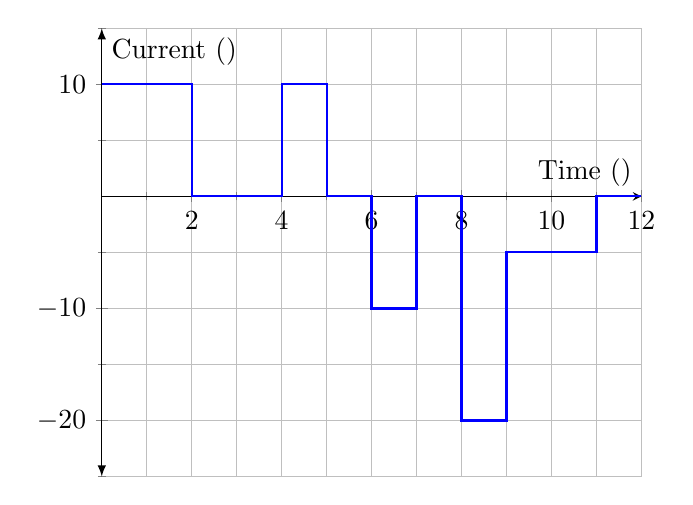
\begin{tikzpicture}
    \begin{axis}[	xmin=0, ymin=-25, xmax=12, ymax=15,
    				xlabel={Time (\si{\second})}, ylabel={Current (\si{\ampere})},
    				legend pos=north west, 
    				domain=0:12,
    				grid=both,
    				axis lines=middle,
    				minor tick num=1,
    				y axis line style={latex-latex}]
        \addplot+[blue, thick, mark=none,const plot]
		coordinates
		{(0,10) (2,10) (2,0) (4,0) (4,10) (5,10) (5,0) (6,0) (6,-10) (7, -10) (7, 0) (8, 0) (8, -20) (9, -20) (9,-5) (11, -5) (11, 0) (12, 0)};
    \end{axis}
	\end{tikzpicture}
	\label{fig:Q3CurrentTime}
\end{center}
\end{solutionorgrid}

\question Given:
\begin{equation*}
	v(t) = 4\sin(3t+4)
\end{equation*}
\begin{parts}
	\part Determine the amplitude of the voltage.
	\begin{solution}[\stretch{1}]
		The amplitude of the voltage can be found by looking at the graph and identifying that the amplitude of the sine wave is \SI{4}{\volt}.
	\end{solution}
	\part The voltage when $t = 1.5$ seconds.
	\begin{solution}[\stretch{1}]
		\begin{equation*}
		\begin{split}
			V & = 4\sin(2\cdot1.5+4)\\
			& = \SI{3.19}{\volt}
		\end{split}
		\end{equation*}
	\end{solution}
\end{parts}
\newpage
\question Given that $R_1 = \SI{2}{\ohm}$ and $R_2 = \SI{3}{\ohm}$, determine the power dissipated by $R_1$ and $R_2$ in Figure~\ref{fig:Q5Circuit}.

\ifprintanswers\else
\begin{center}
\begin{circuitikz}
	\draw
	(0,4)	to[american voltage source, l_=6<\volt>] (0,0)
			to[short] (4,0)
			to[R, l_=$R_2$] (4,4)
			to[short] (0,4)
	(2,0)	to[R, l_=$R_1$] (2,4)
	;
\end{circuitikz}
\captionof{figure}{}
\label{fig:Q5Circuit}
\end{center}
\fi
\begin{solution}
	\begin{multicols}{2}
	Finding total values:
	\begin{equation*}
	\begin{split}
		\frac{1}{R_T} & = \frac{1}{R_1} + \frac{1}{R_2}\\
		& = \frac{1}{2} + \frac{1}{3}\\
		& = \frac{5}{6}\\
		\therefore R_T & = \SI{1.2}{\ohm}\\
		\\
		I_T & = \frac{V}{R_T}\\
		& = \frac{6}{1.2}\\
		& = \SI{5}{\ampere}
	\end{split}
	\end{equation*}
	By current divider law:
	\begin{equation*}
	\begin{split}
		I_{R_1} & = \frac{R_2}{R_1+R_2}\cdot I_T\\
		& = \frac{3}{2+3}\cdot5\\
		& = \SI{3}{\ampere}\\
		\\
		I_{R_2} & =\frac{R_1}{R_1+R_2}\cdot I_T\\
		& = \frac{2}{2+3}\cdot5\\
		& = \SI{2}{\ampere}
	\end{split}
	\end{equation*}
	Now solve the power:
	\begin{equation*}
	\begin{split}
		P_{R_1} & = I^2R_1\\
		& = 3^2\cdot2\\
		& = \SI{18}{\watt}\\
		\\
		P_{R_2} & = I^2R_2\\
		& = 2^2\cdot3\\
		& = \SI{12}{\watt}
	\end{split}
	\end{equation*}
	\end{multicols}
\end{solution}



\question Given the circuit in Figure~\ref{fig:} where $v_s(t)=6\cos(2\pi t)$:
\ifprintanswers\else
\begin{center}
\begin{circuitikz}\draw
	(0,3)	to[american voltage source, l_=$v_s(t)$] (0,0)
			to[short] (2,0)
			to[R, l_=2<\ohm>] (2,3)
			to[short] (0,3)
	;
\end{circuitikz}
\end{center}
\fi
\begin{parts}
	\part Find an expression for the power dissipated in the resistor as a function of time.
	\begin{solution}
		\begin{equation*}
		\begin{split}
			P & = \frac{V^2}{R}\\
			& = \frac{\left(6\cos(2\pi t)\right)^2}{2}\\
			& = 18\cos^2(2\pi t)
		\end{split}
		\end{equation*}
	\end{solution}

	\part Find an equation for the energy dissipated in the resistor as a function of time, given that for $t<0$ there was zero energy dissipation and $v_s(t) = 0$
	\begin{solution}
		\begin{equation*}
		\begin{split}
			E & = \int_0^t P(\tau)\dd{\tau}\\
			& = \int_0^t 18\cos^2(2\pi t)\dd{\tau}
		\end{split}
		\end{equation*}
		Using the trigonometric identity: $\cos(2\theta) = 2\cos^2(\theta) -1$:
		\begin{equation*}
		\begin{split}
			E & = 18\int_0^t\frac{\cos(4\pi t)+1}{2}\dd{\tau}\\
			& = 9\int_0^t\cos(4\pi t)+1\dd{\tau}\\
			& = 9\left[\frac{1}{4\pi}\sin(4\pi t)+\tau\right]^{\tau=t}_{\tau=0}\\
			& = 9\left[\left(\frac{1}{4\pi}\sin(4\pi t)+t\right)-\left(\frac{1}{4\pi}\sin(0)-0\right)\right]\\
			& = \frac{9}{4\pi}\sin(4\pi t) +9t
		\end{split}
		\end{equation*}
	\end{solution}
\end{parts}

\question Consider the circuit in Figure~\ref{fig:Q7Circuit}. Given the power dissipated from $R_1$ is \SI{20}{\watt} and the power dissipated from $R_2$ is \SI{15}{\watt} determine the resistance values of $R_1$ and $R_2$.
\ifprintanswers\else
\begin{center}
\begin{circuitikz}
	\draw
	(0,4)	to[american voltage source, l_=6<\volt>] (0,0)
			to[short] (4,0)
			to[R, l_=$R_2$] (4,4)
			to[short] (0,4)
	(2,0)	to[R, l_=$R_1$] (2,4)
	;
\end{circuitikz}
\captionof{figure}{}
\label{fig:Q7Circuit}
\end{center}
\fi
\begin{solution}
	\begin{equation*}
	\begin{split}
		R & = \frac{V^2}{P}\\
		R_1 & = \frac{6^2}{20}\\
		& = \SI{1.8}{\ohm}\\
		R_2 & = \frac{6^2}{15}\\
		& = \SI{2.4}{\ohm}
	\end{split}
	\end{equation*}
\end{solution}

\question In Figure~\ref{fig:}, given that the voltage across $R_1$ is \SI{4}{\volt}:
\ifprintanswers\else
\begin{center}
\begin{circuitikz}
	\draw
	(0,4)	to[american voltage source, l_=40<\volt>] (0,0)
			to[R, l_=2<\ohm>] (3,0)
			to[short] (6,0)
			to[twoport, t=load] (6,4)
			to[R, l_=$R_1$, i^<=2<\ampere>] (3,4)
			to[R, l_=3<\ohm>, i<_=5<\ampere>] (0,4)
	(3,0)	to[R, l_=5<\ohm>, i^<=3<\ampere>] (3,4)
	;
\end{circuitikz}
\captionof{figure}{}
\label{fig:Q5Circuit}
\end{center}
\fi
\begin{parts}
	\part The power consumed by the resistive load.
		\begin{solution}
			The power generated by the voltage source should equal the power dissipated by both of the resistors and the power consumed by the load, to obey the Law of Conservation of Energy. So, we can find the power generated/consumed by each element allowing us to find the power consumed by the load.
				\begin{equation*}
				\begin{split}
					P_{V_S} & = VI\\
					& = 40\cdot5\\
					& = \SI{200}{\watt}
				\end{split}
				\end{equation*}

				\begin{equation*}
				\begin{split}
					P_{R_1} & = VI\\
					& =  4\cdot2\\
					& = \SI{8}{\watt}
				\end{split}
				\end{equation*}

				\begin{equation*}
				\begin{split}
					P_{\SI{3}{\ohm}} & = i^2R\\
					& = 5^2\cdot3\\
					& = \SI{75}{\watt}
				\end{split}
				\end{equation*}

				\begin{equation*}
				\begin{split}
					P_{\SI{5}{\ohm}} & = i^2R\\
					& = 3^2\cdot5\\
					& = \SI{45}{\watt}
				\end{split}
				\end{equation*}

				\begin{equation*}
				\begin{split}
					P_{\SI{2}{\ohm}} & = i^2R\\
					& = 5^2\cdot2\\
					& = \SI{50}{\watt}
				\end{split}
				\end{equation*}

				\begin{equation*}
				\begin{split}
					P_\text{generated}& = P_\text{consumed}\\
					P_{V_S} & = P_{R_1} + P_{\SI{3}{\ohm}} + P_{\SI{5}{\ohm}} +P_{\SI{2}{\ohm}} + P_\text{load}\\
					P_\text{load} & = 200 - 8 - 75 - 45 - 50\\
					& = \SI{22}{\watt}
				\end{split}
				\end{equation*}

		\end{solution}
	\part The value of $R_1$ and the voltage across the load.
\end{parts}

\end{questions}

